\section{Systems Engineering Considerations}
\label{sec:systems_engineering}

\subsection{Power Budget of the Readout Electronics}
\label{sec:power_budget}
This power budget (see tab. \ref{tab:power_budget}) is based on the power consumption in the data sheets of the electronic components used in the design.
The power consumption of the FPGA is a large estimate, since it depends on the implemented logic.
Also the DRS's power consumption is an estimate based on the value given in a book\footnote{Typical specifications for pixel chips used in particle physics: Power dissipation per pixel \textless $50\mu m$.\cite{rossi2006pixel}}, the real value will depend on the final design.
\begin{table}[H]
	\centering
    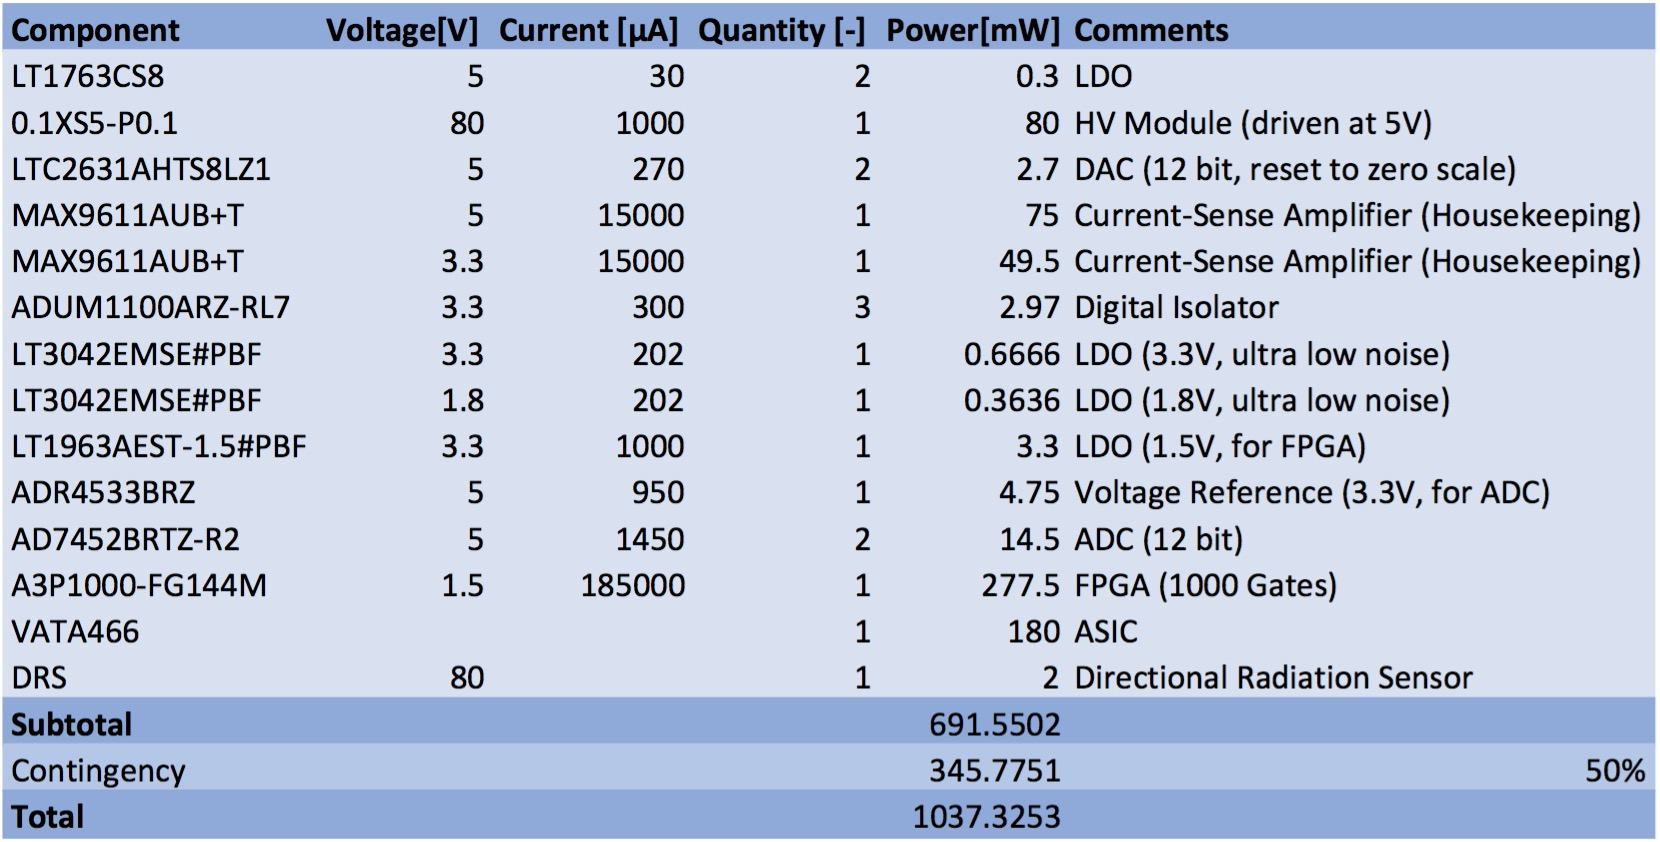
\includegraphics[width=1\textwidth]{power_budget.jpg}
    \caption[Power Budget]{Power budget of the DRS electronics.}
	\label{tab:power_budget}
\end{table}

The budget seems to be realistic, since the total consumed power is close to the 0.9W\cite[p. 11, tab. 4]{tantalumproject2016} of the RADEM mission, which uses a similar DRS.

\subsection{Data Rate and digital resources}
Based on the timing behavior of the FPGA hardware (see fig. \ref{fig:Simulation}) as well as the operating clock frequencies of the interfaces, the maximum data rate generated by the directional radiation sensor through the readout electronics can be estimated. 

\begin{table}[H]
	\centering
    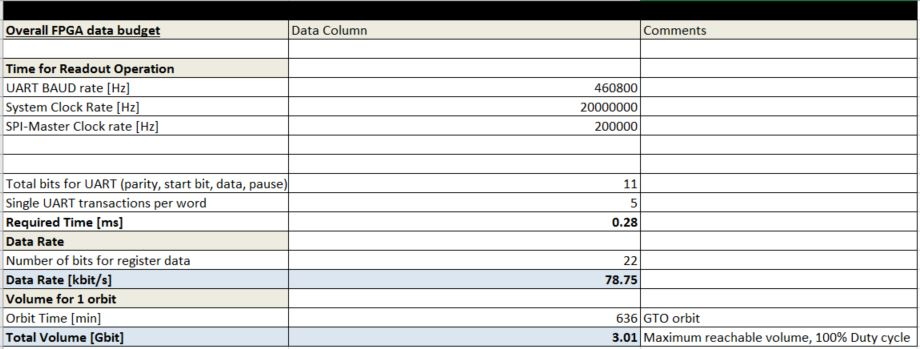
\includegraphics[width=1\textwidth]{Data_budget.JPG}
    \caption[Data Budget]{Maximum data rate and data volume of FPGA sensor readout operation.}
	\label{tab:data_budget}
\end{table}

Another important consideration are the available hardware gate resources on the FPGA. In the Libero SoC software, the required digital resources can be estimated.

\begin{table}[H]
	\centering
    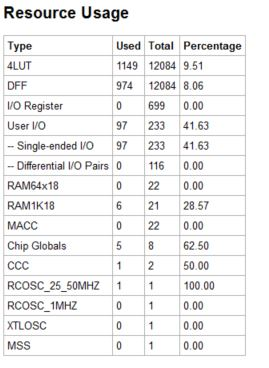
\includegraphics[width=0.2\textwidth]{resource.JPG}
    \caption[Components]{Share of hardware components used for the synthesis of the design on the SmartFusion2 M2S050}
	\label{tab:resource}
\end{table}

These figures can be compared to the hardware resources of the current choice for the FPGA.

\begin{table}[H]

\caption[]{UART Core specifications \cite{Actel}}
    \label{tab:11}
    
  \begin{center}  
  \begin{tabular}{|r|l|}
  \hline
  \textbf{Part}  & \textbf{ProASIC3 A3P1000} \\ \cline{1-2}
  
  \textbf{System Gates} & 1 Million \\
  \textbf{D-Flip-Flops} & 24576\\ 
  \textbf{RAM Kbits} & 144 \\
  \textbf{FlashROM} & 1K\\
  \textbf{Integrated PLL} & 1 \\
  \textbf{Global Signals} & 18 \\
  \textbf{I/O Banks} & 4 \\
  \textbf{Single-Ended I/Os} & 154 \\
  \textbf{Differential I/O Pairs} & 35 \\
  \hline
  
\end{tabular}
\end{center}
\end{table}

If the DFF (D-Flip-Flop) count between the existing design and the available resources for the ProASIC3, it becomes evident, that there is a passable margin between the required and 


\subsection{Radiation tolerance of the ProASIC3 A3P1000}

\subsection{\texorpdfstring{$I^2C$}{TEXT} Interfaces}
\label{sec:i2c_interfaces}
Some electric components in the design can only be accessed via an $I^2C$ interface. 
Their addresses are defined in the following table:
\begin{table}[H]
	\centering
    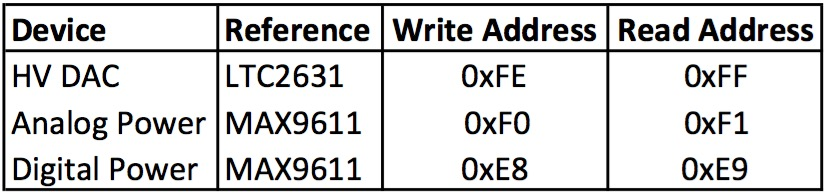
\includegraphics[width=0.5\textwidth]{i2c_interfaces.jpg}
    \caption[$I^2C$ Interfaces]{$I^2C$ interface addresses.}
	\label{tab:i2c_interfaces}
\end{table}
